\documentclass{iopart}

\usepackage{url}
\usepackage{amsbsy}
\usepackage{graphicx}
\usepackage[usenames]{color}
\usepackage{iopams}
\usepackage{epstopdf}

\newcommand{\eqref}[1]{{(\ref{#1})}}
\newcommand{\ilya}[1]{{\color{red} \bf Ilya: #1}}
 

\begin{document}

\title{Report on the third Mock LISA Data Challenge} 

\author{The \emph{Mock LISA Data Challenge Task Force}:
\ilya{Both lists need updating: }
Stanislav Babak$^1$,
John G. Baker$^2$,
Matthew J. Benacquista$^3$,
Neil J. Cornish$^4$,
Jeff Crowder$^5$,
Curt Cutler$^{5,6}$,
Shane L. Larson$^7$,
Tyson B. Littenberg$^4$,
Edward K. Porter$^1$,
Michele Vallisneri$^{5,6}$,
Alberto Vecchio$^{8,9}$ and \emph{the Challenge-3 participants}:
Gerard Auger$^{10}$,
Leor Barack$^{11}$,
Arkadiusz B\l aut$^{12}$,
Ed Bloomer$^{13}$,
Duncan A. Brown$^{14,15,6}$,
Nelson Christensen$^{16}$,
James Clark$^{13}$,
Stephen Fairhurst$^{17,15,6}$,
Jonathan R. Gair$^{18}$,
Hubert Halloin$^{10}$,
Martin Hendry$^{13}$,
Arturo Jimenez$^3$,
Andrzej Kr\'olak$^{19}$,
Ilya Mandel$^{9,6}$,
Chris Messenger$^{13}$,
Renate Meyer$^{20}$,
Soumya Mohanty$^3$,
Rajesh Nayak$^3$,
Antoine Petiteau$^{10}$,
Matt Pitkin$^{13}$,
Eric Plagnol$^{10}$,
Reinhard Prix$^1$,
Emma L. Robinson$^1$,
Christian Roever$^{20}$,
Pavlin Savov$^{6}$,
Alexander Stroeer$^{8,9}$,
Jennifer Toher$^{13}$,
John Veitch$^8$,
Jean--Yves Vinet$^{21}$,
Linqing Wen$^1$,
John T. Whelan$^{22}$,
Graham Woan$^{13}$}
\address{$^1$ Max-Planck-Institut f\"ur Gravitationsphysik (Albert-Einstein-Institut), Am M\"uhlenberg 1, D-14476 Golm bei Potsdam, Germany}
\address{$^2$ Gravitational Astrophysics Lab., NASA Goddard Space Flight Center, 8800 Greenbelt Rd., Greenbelt, MD 20771, USA}
\address{$^3$ Center for Gravitational Wave Astronomy, Univ.\ of Texas at Brownsville, Brownsville, TX 78520, USA}
\address{$^4$ Dept.\ of Physics, Montana State Univ., Bozeman, MT 59717, USA}
\address{$^5$ Jet Propulsion Laboratory, California Inst.\ of Technology, Pasadena, CA 91109, USA}
\address{$^6$ Theoretical Astrophysics, California Inst.\ of Technology, Pasadena, CA 91125}
\address{$^7$ Dept.\ of Physics, Weber State Univ., 2508 University Circle, Ogden, UT 84408, USA}
\address{$^8$ School of Physics and Astronomy, Univ.\ of Birmingham, Edgbaston, Birmingham B152TT, UK}
\address{$^9$ Dept.\ of Physics and Astronomy, Northwestern Univ., Evanston, IL, USA}
\address{$^{10}$ APC, UMR 7164, Univ.\ Paris 7 Denis Diderot, 10, rue Alice Domon et Leonie Duquet, 75025 Paris Cedex 13, France}
\address{$^{11}$ School of Mathematics, Univ.\ of Southampton, Southampton, SO171BJ, UK}
\address{$^{12}$ Inst.\ of Theoretical Physics, Univ.\ of Wroc\l aw, Wroc\l aw, Poland}
\address{$^{13}$ Dept.\ of Physics and Astronomy, Univ.\ of Glasgow, Glasgow, UK}
\address{$^{14}$ Dept.\ of Physics, Syracuse Univ., Syracuse, NY13244, USA}
\address{$^{15}$ LIGO Laboratory, California Inst.\ of Technology, Pasadena, CA 91125}
\address{$^{16}$ Physics and Astronomy, Carleton College, Northfield, MN, USA}
\address{$^{17}$ School of Physics and Astronomy, Cardiff Univ., 5, TheParade, Cardiff, UK, CF243YB}
\address{$^{18}$ Inst.\ of Astronomy, Univ.\ of Cambridge, Cambridge, CB30HA, UK}
\address{$^{19}$ Inst.\ of Mathematics, Polish Academy of Sciences, Warsaw, Poland}
\address{$^{20}$ Dept.\ of Statistics, The Univ.\ of Auckland, Auckland, New Zealand}
\address{$^{21}$ ARTEMIS, Observatoire de la Cote d'Azur-C.N.R.S., 06304 Nice, France} 
\address{$^{22}$Center for Computational Relativity and Gravitation and School of Mathematical Sciences, Rochester Institute of Technology, 85 Lomb Memorial Drive, Rochester, NY 14623, USA}

\ead{Michele.Vallisneri@jpl.nasa.gov}

\begin{abstract}
This be the abstract
%The Mock LISA Data Challenges are a program to demonstrate LISA data-analysis capabilities and to encourage their development. Each round of challenges consists of several data sets containing simulated instrument noise and gravitational waves from sources of undisclosed parameters. Participants are asked to analyze the data sets and report the maximum information about the source parameters. The challenges are being released in rounds of increasing complexity and realism: here we present the results of Challenge 2, issued in Jan 2007, which successfully demonstrated the recovery of signals from nonspinning supermassive--black-hole binaries with optimal SNRs between $\sim 10$ and $2000$, from $\sim 20,000$ overlapping Galactic white-dwarf binaries (among a realistically distributed population of 26 million), and from the extreme--mass-ratio inspirals of compact objects into central galactic black holes with optimal SNRs $\sim 100$.
\end{abstract}

\vspace{-18pt}
\pacs{04.80.Nn, 95.55.Ym}

\maketitle

\section{Introduction}

%The Laser Interferometer Space Antenna (LISA), a NASA and ESA space mission to detect gravitational waves (GWs) in the $10^{-5}$--$10^{-1}$ Hz range \cite{lisa}, will produce time series consisting of the superposition of the signals from millions of sources, many in our Galaxy, some as far as the edge of the observable universe. Some of the signals, such as those from extreme--mass-ratio inspirals (EMRIs), are very complex functions of the source parameters; others, such as those from Galactic white-dwarf binaries, are simpler, but their resolution will be confused by the presence of many other similar signals that overlap in frequency space. Thus, data analysis is integral to the LISA measurement concept, because no source can be observed without first carefully teasing out its individual voice in the noisy party of the LISA data. Indeed, it is important to understand data analysis in order to demonstrate that LISA can meet its science requirements, and to translate these into decisions on instrument design.

%The idea of the Mock LISA Data Challenges (MLDCs) arose in late 2005 from this very realization. The MLDCs have the purpose of encouraging and tracking progress in LISA data-analysis development, and (as a useful byproduct) of producing a prototype of the LISA computational infrastructure, including common data formats, standard models of the LISA orbits, noises and measurements, software tools to generate waveforms and to simulate the LISA response, and more.
%The MLDCs are a coordinated (but voluntary) effort in the GW community, whereby a task force chartered by the LISA International Science Team periodically issues data sets containing synthetic noise and GW signals from sources of undisclosed parameters; challenge participants return detection candidates and parameter estimates, together with descriptions of their search methods. These results are then compiled and compared to the previously secret challenge ``key.''

%Challenge 1, issued in Jun 2006 with results due in Dec 2006 (see \cite{mldclisasymp,mldcgwdaw1}), tackled the detection and parameter characterization of \emph{verification binaries} (Galactic binaries of known frequency and position); of loud unknown Galactic binaries, either alone or in small, moderately interfering groups; and of relatively loud inspirals of nonspinning supermassive--black-hole (MBH) binaries. All sources were represented by somewhat idealized waveforms, and they were staged on simulated instrument noise alone. Ten collaborations submitted entries, adopting a variety of methods (template-bank, stochastic- and genetic-optimization matched filtering; time--frequency; tomography; Hilbert transform). Despite the short timescale, each challenge was ``solved'' by at least one group, although some searches locked on strong secondary probability maxima for the source parameters. More important, Challenge 1 helped set the playing field and assemble the computational tools for the more realistic Challenge 2.

%Challenge 2, issued in Jan 2007 with results due at the end of Jun 2007, raised the bar by proposing three complex subchallenges. Data set 2.1 contained signals from a full population of Galactic binary systems (about 26 million sources). Data set 2.2 contained signals from a similar (but distinct) Galactic-binary population, plus an undisclosed number (between 4 and 6) of signals from nonspinning-MBH binary inspirals with optimal single-interferometer signal-to-noise ratios (SNRs) between 10 and 2000 and a variety of coalescence times, and plus five EMRI signals with optimal SNRs between 30 and 100. The EMRIs were modeled as Barack and Cutler's ``analytic kludges'' \cite{barackcutler}: adiabatic sequences of elliptical orbits emitting Peters--Mathews waveforms, with separation, precession and eccentricity evolving according to post-Newtonian equations. Last, five more data sets (denoted 1.3.1--5, since they were released at the time of Challenge 1) contained single EMRI signals over instrument noise alone, with optimal SNRs between 40 and 110. See \cite{mldcgwdaw2} for more details about the signal models and the ranges from which the source parameters were drawn.

%Thirteen collaborations (comprising all the researchers listed as participants in the byline of this article, and most task force members) submitted a total of 22 entries, including a proof-of-principle analysis for stochastic backgrounds performed on data set 2.1.
%Altogether, Challenge 2 successfully demonstrated the identification of $\sim 20,000$ Galactic binaries, the accurate estimation of nonspinning-MBH inspiral parameters, and the positive detection of EMRIs, as we discuss in more detail in the rest of this paper. All the solutions submitted by participating groups, together with technical write-ups of their methods and findings, can be found at the URL \url{www.tapir.caltech.edu/~mldc/results2}. A few groups are also contributing descriptions of their work to the proceedings of this conference.

\section{Challenge 3.1: The Galactic Binaries {\it Neil and Matt}}

\section{Challenge 3.2: The Massive Black Hole Binaries {\it Antoine}}
The data set 3.2 contained four to six signals from the inspiralling spinning Massive Black Hole (MBH) binaries embedded in the instrument noise and Galactic background. The Galactic background was modeled as simulated 
Galactic GW data with signals below signal-to-noise ratio 6. 
For signal from the spinning MBH binaries in the quasi-circular orbit we have adopted the restricted waveforms with 
the GW phase up to 2 Post-Newtonian order (see section 3.2 of \cite{MLDC3}). The magnitude and orientation of spins cover all possible values.  Each source is described by fifteen parameters: the two masses $m_{1}$ and $m_{2}$, the time of coalescence $t_{c}$, the sky-position $\beta$ and $\lambda$, the luminosity distance $D_{L}$, the initial orbital phase $\phi_{0}$, the magnitude of spins $a_{1}$ and $a_{2}$, the initial orientation of the first spin  $\theta_{S1}$ and $\phi_{S1}$, the orientation of the second spin $\theta_{S2}$ and $\phi_{S2}$ and the initial orientation of the orbital angular momentum  $\theta_{L}$ and $\phi_{L}$. The parameters for all sources are drawn uniformly from the 
same prior range, but were distinguished by the times of coalescence and the SNR which are given in Table 8 of \cite{MLDC3}.

The participants could submit multiple modes for each sources provided that there was no clear way to prefer one to another, in other words, the solutions should reflect the degeneracies in the parameter space and multi-modality of the
likelihood. Five groups submitted their results: 
\begin{itemize}
\item \textbf{AEI} (Albert Einstein Institute (Germany))  have used a matched-filtering based genetic algorithm extended to a multi-modal search. The maximized function is {\em A-statistic} which is a geometrical mean of the log-likelihood for the whole duration of template and the low-frequency template \cite{GAspinbbhFullPaper}.

\item \textbf{CambAEI} (collaboration between Cavendish Laboratory (UK), the Institute of Astrophysics (UK) and Albert Einstein Institute, (Germany)) have employed MultiNest algorithm \cite{MultiNest2} to compute the 
evidence and to produce posterior distribution. The method is intrinsically multi-modal as it name states. They have 
also used {\em A-statistic} to identify modes.

\item \textbf{MTGWAGAPC} (a collaboration between Montana Gravitational Wave Astronomy Group (US) and  
Astro-Particle and Cosmology Institut (France)) have used a parallel tempering MCMC algorithm. It is based on the MHMC algorithm used in previous challenges which utilizes frequency and thermostated annealing for an efficient parameter space exploration \cite{SMBHCornishPorter}. Parallel tempering employs a number of chains
 at different temperatures where the hot chains explore the parameter space throughout the whole range, while the cool chains concentrate on the local maxima and the chains exchange information with each other.

\item \textbf{JPLCITNWU} (a collaboration between  CalTech (US),  Jet Propulsion Laboratory (US)  
the Northwester University (US)) have employed a two-stage method. At first, they have searched for the bright sources using the tools developed for the non-spinning MBH search \cite{JPLCaltech}, and in the second stage, they have employed  MultiNest algorithm.

\item \textbf{GSFC} (Goddard Space Fly Center (US)) used a tempered Metropolis-Hastings MCMC algorithm within the framework of Xspec \cite{Xspec}. 

\end{itemize}

There were five signals from MBH binaries in this data set. The first three binaries which coalesce within the 
observation (MBH-1, 3 and 4) were detected by all five groups except MBH-4 for GSFC (we consider a result as a detection if $SNR > 5$ with $t_{c}$ close to the true value). From last two low SNR signals, MBH-2 (SNR $\sim$ 19) was detected by AEI, CambAEI, MTGWAGAPC and JPLCITNWU, whereas MBH-6 (SNR $\sim$ 13) was positively detected only by two groups, AEI and CambAEI.  

The Table \ref{tab:SMBH_Err} shows fractional errors in the parameters estimation for the five sources. We have chosen only the best mode from each submission (i.e. highest SNR) for comparison with the true solution. Note that 
sometimes the difference in the SNR of several modes was less that one (sigma), and the mode with the better 
parameters recovery was not chosen.
Table \ref{tab:SMBH_SNR} shows the recovered SNR and the overlap with  the true waveform for TDI channels A and E. The waveforms for the SNR and overlap evaluation were constructed using the submitted parameters and the software
used to produce MLDC.

\begin{table}
\begin{center}
\begin{tabular}{lr|rrrrrrr}
\hline
Source & group & $\Delta M_{c}/ M_{c}  $& $\Delta \eta/ \eta $ & $ \Delta t_{c} $ &  $ \Delta $ Sky  & $ \Delta a_{1} $ & $ \Delta a_{2}  $ &  $\Delta D / D$ \\
 & & $\times 10^{-5}$ & $\times 10^{-4}$ & (sec) & (deg) & $\times 10^{-3}$ & $\times 10^{-3}$ & $\times10^{-2}$   \\

\hline
             & AEI            &         2.4 &        6.1 &   62.9 &   11.6 &    7.6 &   47.4 &   8.0 \\
             & CambAEI &         3.4 &     40.7 &   24.8 &      2.0 &    8.5 &   79.6 &   0.7    \\
MBH-1 & MTAPC    &       24.8 &     41.2 & 619.2 & 171.0 & 13.3 &   28.7 &    4.0  \\
              & JPL           &       40.5 &  186.6 &   23.0 &    26.9 & 39.4 &   66.1 &    6.9  \\
              & GSFC       &  1904.0 &  593.2 & 183.9 &    82.5 &   5.7 & 124.3 &  94.9  \\

\hline
               & AEI            &       9.0 &         5.2 &    100.8 & 175.9 &      6.2 &    18.6 &   2.7  \\
               & CambAEI &     13.5 &      57.4 &    138.9 & 179.0 &    21.3 &      7.2 &   1.5 \\
MBH-3  & MTAPC    &   333.0 &    234.1 &    615.7 &   80.2 &    71.6 & 177.2 & 16.1  \\
               & JPL           &   153.0 &      51.4 &    356.8 &   11.2 & 187.7 & 414.9 &    2.7  \\
               & GSFC       & 8168.4 & 2489.9 & 3276.9 &    77.9 & 316.3 &   69.9 &  95.6 \\

\hline
                & AEI            &      4.5 &      75.2 &       31.4 &   0.1 & 47.1 &173.6  &    9.1 \\
                & CambAEI &      3.2 &    171.9 &      30.7 &   0.2 & 52.9 & 346.1 &  21.6 \\
MBH-4   & MTAPC    &     48.6 & 2861.0 &        5.8 &   7.3 & 33.1 & 321.1 & 33.0  \\
                & JPL           &  302.6 &    262.0 &   289.3 &   4.0 & 47.6 & 184.5 & 28.3  \\
                & GSFC       &  831.3 & 1589.2 & 1597.6 & 94.4 & 59.8 & 566.7 & 95.4  \\

\hline
                & AEI            & 1114.1 & 952.2 & 38160.8 & 171.1 & 331.7 & 409.0 &  15.3 \\
MBH-2   & CambAEI &      88.7 & 386.6 &   6139.7 & 172.4 & 210.8 & 130.7 &  24.4  \\
                & MTAPC    &   128.6 &   45.8 & 16612.0 &      8.9 & 321.4 & 242.4 &  13.1  \\
                & JPL           &   287.0 & 597.7 & 11015.7 &   11.8 & 375.3 & 146.3 &    9.9 \\

\hline
                & AEI            &    1042.3 & 1235.6 &   82343.2 &      2.1 & 258.2 & 191.6 & 26.0  \\
MBH-6   & CambAEI &    5253.2 & 1598.8 & 953108.0 & 158.3 & 350.8 & 215.4 & 29.4  \\
                & MTAPC    & 56608.7 &    296.7 & 180458.8 & 119.7 & 369.2 & 297.6 & 25.1  \\


\hline
\end{tabular}
\end{center}
\caption{ Relative/absolute errors for the spinning MBH binaries in Challenge~3.2. All parameters are defined as in the table 7 of \cite{MLDC3}, except for the chirp mass $M_c \equiv (m_1 m_2)^{3/5} / (m_1 + m_2)^{1/5}$ and for the symmetric mass ratio $\eta = m_1 m_2 / (m_1 + m_2)^{2}$.  $ \Delta \textmd{Sky}$ is the angular distance in the sky between 
the true and the estimated positions. We used only the mode with the highest SNR in all tables, if several modes per group were submitted.
\label{tab:SMBH_Err}}
\end{table} 


\begin{table}
\begin{center}
\begin{tabular}{lr|rrrrr}
\hline
Source                              & group &  MBH-1      & MBH-3   & MBH-4    & MBH-2 & MBH-6   \\
($\textrm{SNR}_{true}$) &              & (1670.58) & (847.61) & (160.05) & (18.63) & (12.82) \\
\hline
                      & AEI            & 1657.71 & 846.96 & 160.05 & 20.54 & 13.69 \\
                      & CambAEI & 1657.19 & 847.04 & 160.02 & 20.36 & 10.17 \\
SNR             & MTAPC    & 1669.97 & 842.96 & 149.98 & 20.27 & 13.36\\
                      & JPL           & 1664.87 & 835.73 & 158.34 & 18.20 & - \\
                      & GSFC       &   267.04 & 218.05 &  -45.53 & - & - \\
\hline
                      & AEI            & 0.9936 & 0.9995 &  0.9989 & 0.9399 &  0.9288 \\
                      & CambAEI & 0.9925 & 0.9993 &  0.9991 & 0.9592 &  0.4018 \\
Overlap A    & MTAPC    & 0.9996 & 0.9943 &  0.8766 & 0.9238 & -0.0037 \\
                      & JPL           & 0.9972 & 0.9826 &  0.8895 & 0.9661 & - \\
                      & GSFC       & 0.1827 & 0.2815 & -0.1725 & - & - \\
\hline
                      & AEI            & 0.9914 & 0.9989 &  0.9994 & 0.9469 &  0.9293 \\
                      & CambAEI & 0.9917 & 0.9993 &  0.9992 & 0.9697 &  0.4399 \\
Overlap E    & MTAPC    & 0.9997 & 0.9945 &  0.9352 & 0.9149 &  0.0375\\
                      & JPL           & 0.9981 & 0.9898 &  0.9925 & 0.9709 & - \\
                      & GSFC       & 0.1426 & 0.2314 & -0.2937 & - & - \\
\hline
\end{tabular}
\end{center}
\caption{ Recovered SNR and overlaps for spinning MBH binaries in Challenge~3.2. The negative
SNR is the result of the negative overlap and corresponds to  the waveforms in anti-phase.
\label{tab:SMBH_SNR}}
\end{table} 

The accuracy in the parameter estimation strongly depends on whether we have observed the coalescence or not.
The signals with observed merger (MBH-1, 3 and 4) have significantly larger SNR and span to higher frequencies, 
allowing much more accurate recovery of the parameters of the MBH binary. 
 For these sources, the errors in the masses, the time at coalescence, the distance and the sky position are comparable, if not better, to the ones obtained in non-spinning case (see table 1 and 2 of report on challenge 2.2 \cite{MLDC2Res}). Concerning the position on the sky, the results with  $\Delta \textrm{Sky} > 170 \deg$, correspond to the mirrored sky location which is a known degeneracy in the response function. The errors in the spin amplitudes
  are consistent with the Fisher matrix prediction \cite{SpinBBHLangHugues}.  Despite the high SNR, the evaluation of the initial direction of the spins and of the orbital angular momentum has proven to be very difficult.  We observe a large number of the local maxima in these parameters which have SNR very close to the true one. This is illustrated in the Figure~\ref{fig:SMBH_spinLdeg} which shows the distribution of $\theta_{S1}$, $\phi_{S1}$, $\theta_{S2}$, $\phi_{S2}$, $\theta_{L}$ and $\phi_{L}$ for all the submitted modes for MBH-3. We see that the modes are well separated in parameters value but a difference in the SNR is less than 10. The SNR of the majority submitted results are within 10 (sigma) of the true one and the overlap is higher than 0.99.
This reflects degeneracies in the parameter space and that the recovered signals resemble the true one very closely, despite poor estimation of some parameters.


\begin{figure}
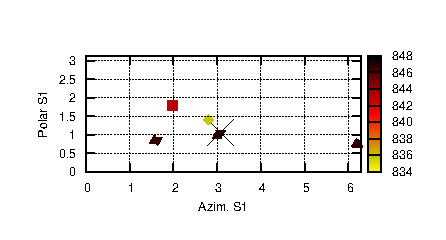
\includegraphics[width=0.5\textwidth, clip=true, viewport=0 4 198 83 ]{DirS1_srcMC2_SNR.eps}
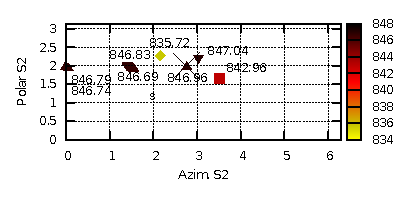
\includegraphics[width=0.5\textwidth, clip=true, viewport=0 4 198 83 ]{DirS2_srcMC2_SNR.eps}\\
\center 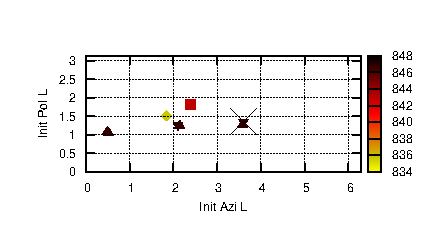
\includegraphics[width=0.5\textwidth, clip=true, viewport=0 4 198 83 ]{DirL_srcMC2_SNR.eps}
\caption{Distribution of the modes for the initial direction of spin 1, spin 2, and orbital angular momentum for source MBH-3 is shown in the top-left, top-right and bottom panels, respectively. The cross corresponds to the true value ($\times$), the triangle up ($\blacktriangle$) are the modes form AEI, the triangle down ($\blacktriangledown$) are the modes form CambAEI, the square ($\blacksquare$) is the mode from MTGWAGAPC and the diamond ($\blacklozenge$) is the mode from JPLCITNWU submission. The color corresponds to the SNR.
\label{fig:SMBH_spinLdeg}}
\end{figure}


Let us now comment on the parameter estimation for the last two signals with the coalescence time beyond the observational time. For MBH-2 the error in the masses and the time of coalescence are comparable to the Fisher matrix predictions. 
The errors in the sky localization is around 10 degrees with a very strong local maximum at the mirrored 
sky position. The overlaps between the recovered waveforms and the true ones are higher than 0.9 for all submissions.
The recovered SNR for some modes was higher than the true one which is an artifact of the evaluation: 
we extend the computation of the inner products beyond the frequency range of the signals which picks up a bit of the 
``junk'' SNR from the correlation with the noise. 
%
The determination of the spin amplitude is very bad. This reflects the fact that the spins have a very weak effect on the low frequency part of the waveform. 

The source MBH-6 was the weakest, and the overlap evaluation suggests that only AEI group made a positive detection. 

The spins are supposed to de-correlate some parameters in the waveform \cite{SpinBBHLangHugues} and we 
might observe this in some cases, but more investigations are needed to clearly conclude on this point.
However, the spins also bring additional degeneracies and multiple local maxima in the parameter space, especially in the initial directions of the spins and the orbital plane. This complexity is reflected in the submitted results.
Nevertheless these results demonstrate solid capability in detecting the signals and good recovery of other 
nine parameters. 




\section{Challenge 3.3: The Extreme Mass Ratio Inspirals {\it Ilya}}

The Extreme-Mass-Ratio Inspiral (EMRI) signals in Challenge 3.3 are based on Barack \& Cutler analytical kludge waveforms \cite{barackcutler}, as described in \cite{mldcgwdaw2}, but with only five harmonics present per signal \cite{MLDC3}.  Five EMRIs were injected, all coalescing during the second year of the data set, with dimensionless spins between $0.5$ and $0.7$, eccentricities at plunge between $0.15$ and $0.25$, and smaller-body masses between $9.5 M_\odot$ and $10.5 M_\odot$.  The mass of the larger body was in the range $0.95$--$1.05\times10^7 M_\odot$ for source 3.3.1,  $4.75$--$5.25 \times10^6 M_\odot$ for sources 3.3.2 and 3.3.3, and $0.95$--$1.05\times10^6 M_\odot$ for sources 3.3.4 and 3.3.5 (see Table 8 of \cite{MLDC3}).  In addition to the presence of multiple sources in the same data stream, the challenge participants had to contend with much weaker signals than in previous EMRI challenges, with announced signal-to-noise ratios varying between $10$ and $50$ (actual blind-injection SNRs varied between $20$ and $37$).

Three groups attempted to find the Challenge 3.3 sources.  These were:
\begin{itemize}
\item \textbf{BabakGair}: This collaboration between AEI and Cambridge University used stochastic sampling and Markov Chain Monte Carlo techniques to find signal harmonics, and then carried out an F-statistic search in the space of harmonics before applying MCMC in the physical parameter space for the final fit.  The basic methodology is described in \cite{BabakGairPorter}, but this search contained several improvements in harmonic identification.
\item \textbf{EtfAG}: This collaboration between Cambridge University and Northwestern University searched the time-frequency spectrogram for harmonics using the Chirp-based Algorithm for Track Search (CATS, \cite{CATS}) which they developed for earlier MLDC rounds \cite{GairMandelWen}; this iteration included several improvements to the search technique to allow for intersecting tracks from multiple sources.
\item \textbf{MTAPCIOA} This collaboration between Montana State University, APC-Paris, and Cambridge University ... {\bf *** To be completed}.
\end{itemize}


\begin{table}
\begin{center}
\begin{tabular}{lr|rrrrrrrr}
\hline
Source & group & SNR & $\Delta M/ M  $ & $\Delta \mu/ \mu $ & $ \Delta t_{c} $ &  $ \Delta  e_0 / e_0 $ & $ \Delta |S| / |S| $ & $ \Delta \lambda / \lambda  $ &  $\Delta D / D$ \\
(true SNR) & & $\times 10^{-3}$ & $\times 10^{-3}$ & (sec) &  &  & &    \\

\hline
EMRI-1& MTAPCIOA  & &  & & & & & &  \\
(21.6732) & MTAPCIOA & & & & & & & &     \\
\hline
EMRI-2& MTAPCIOA & & & & & & & &  \\
(33.3534)    & BabakGair & & & & & & & &     \\    
              & BabakGair & & & & & & & &     \\    
              & BabakGair & & & & & & & &     \\       
              & EtfAG & & & & & & & & \\  
\hline
EMRI-3& MTAPCIOA & & & & & & & &  \\
(20.9811)  & BabakGair & & & & & & & &     \\    
             & BabakGair & & & & & & & &     \\    
              & BabakGair & & & & & & & &     \\        
\hline
EMRI-4& MTAPCIOA &  &  & & & & & &  \\
(26.6500)  & MTAPCIOA & & & & & & & &     \\
\hline
EMRI-5& MTAPCIOA  & &  & & & & & &  \\
(36.1731) & MTAPCIOA & & & & & & & &     \\
\hline                                               


\end{tabular}
\end{center}
\caption{Parameter estimation errors for the EMRIs in Challenge~3.3. All parameters are defined as in the table 5 of \cite{mldcgwdaw2}.
%We used only the mode with the highest SNR in all tables, if several modes per group were submitted.
\label{tab:EMRI_Err}}
\end{table} 

The MLDC 3.3 parameter-estimation results are presented in Table \ref{tab:EMRI_Err}.
{\bf *** To be completed}

\section{Challenge 3.4: The Cosmic String Cusp Bursts {\it Ed}}

A new source for Challenge 3 is the gravitational radiation emitted from the cusps of cosmic superstrings.  The blind data was composed of a one month data set (i.e. $2^{21}$ samples at 1 second cadence) and contained 3 such sources.  Each source is described
by a set of 6 parameters : the ecliptic latitude $\beta$ and longitude $\lambda$, the amplitude of the wave ${\mathcal A}$, the polarization of the wave $\psi$, the burst's
central time of arrival $t_C$ and a frequency parameter $f_{max}$.  This is the frequency beyond which there is a significant decay in the power spectrum of the burst, and is related to both the characteristic lengthscale of the string and the viewing angle.

The groups were informed that the signal to noise ratio was uniform between 10 and 100, the logarithm of ($f_{max}/$Hz) was uniformly distributed between $[-3,1]$ and the event rate was Poisson distributed with 5 events per month.  Four groups returned entries for Challenge 3.4 .  These were
\begin{itemize}
\item \textbf{CAM} :  A collaboration between Cambridge University and APC-Paris using the MultiNest algorithm. This is an efficient multi-modal
Nested Sampling search algorithm which uses a number of live points in the parameter space.  
\item \textbf{CaNoe} : A collaboration between Cambridge University and Northwestern University using a Time-Frequency search algorithm. This algorithm is a modified
version of the Chirp-based Algorithm for Track Searches which identifies tracks of a particular shape in the spectrogram.
\item \textbf{JPLCIT} : A JPL-Caltech collaboration which used both Markov Chain Monte Carlo (MCMC) and MultiNest algorithms.  The results presented here are for 
the MultiNest search only.
\item MTGWAG : The GW group at Montana State University used a parallel tempered MCMC technique~\cite{keycornish}.  The MCMC is a stochastic search method which is particularly
useful for searches conducted in high dimensional spaces.  The parallel tempering adds the complexity of a number of inter-communicating search
chains at different temperatures.
\end{itemize}

The four groups were successful in recovering all three burst sources.  In Table~\ref{tab:parerrs} we present the errors in parameter estimation for each group.  As each burst is of relatively short duration, LISA can be taken as being an effectively static detector.  Because of this, the position of the source in the sky is harder to determine than for other sources.  It has also been shown~\cite{keycornish} that for cosmic string bursts there are a number of degeneracies in the parameter space.  For example, a reflection in the plane of the detector produces one set of degenerate parameters, while a rotation in the plane generates two sets of secondary maxima.  This coupled with the fact that there is a high correlation between the sky position of the source and the central burst time makes parameter estimation very difficult.  

We can see in most cases that the errors for the ecliptic latitude $\beta$ are between 0.1 and 1 radians, while the errors in the estimation of the longitude are much bigger.  This inaccuracy in the sky position also makes it difficult to determine the polarization of the wave.  In certain cases, the errors in sky resolution translates to a large error in the estimation in the central burst time $t_C$.   Similarly, groups had trouble determining the value of $f_{max}$ and in some cases returned the value of the Nyquist frequency in their search (i.e. 0.5 Hz) which resulted in the occasionally very large errors in the estimation of this parameter. Finally, in most cases the groups were able to resolve the amplitude of the waves.

\begin{table}
\caption{\label{tab:parerrs}Returned values for cosmic string search.  Some groups returned multiple mode solutions, which are also presented.  The dashed lines represent unreturned parameter values.  The angular errors have units of radians.} 
\vspace{2mm}
%\begin{indented}
%\lineup
%\item[]
%\begin{tabular}{@{}*{8}{l}}
\lineup
%\scriptsize 
\flushright
\begin{tabular}{llllllll}
\br                              
Group& \centre{1}{source}& \centre{1}{$\Delta\beta$}&\centre{1}{$\Delta\lambda$}&\centre{1}{$\Delta\psi$}&\centre{1}{$\Delta{\mathcal A}/{\mathcal A}$}&\centre{1}{$\Delta t_C/t_C$}&\centre{1}{$\Delta f_{max}/f_{max}$}\cr 
\br
CAM&1& \m1.118 & $-1.745$& \m2.393& $-0.319$& \m0.626& $-15.896$\cr
&& \m0.298 & $-0.277$& \m1.195& $-0.220$& \m0.626& $-15.896$\cr
&& $-0.432$ & \m3.029& \m 3.658& \m0.674&\m0.441& $-460.157$ \cr
&2& \m0.449 & $-1.949$& \m4.846& $-0.062$& $-4.638\times10^{-4}$&\m$3.399\times10^{-3}$ \cr
&3& $-1.149$ &$ -5.794$& \m1.843&$ -0.932$& $-1.672$& \m0.919\cr
&& $-1.733$ & $-4.747$& \m2.408& $-1.159$& $-1.671$& \m0.919\cr
\mr
CaNoE&1& \m---& \m---& \m---& $-0.154$& \m0.626& $-15.896$ \cr 
&2&\m ---& \m---& \m---& \m0.642& $-4.137\times10^{-4}$& $-0.199$ \cr 
&3&\m ---&\m ---& \m---&  $-0.171$& $-1.671$& \m0.919 \cr 
\mr
JPLCIT&1& \m0.353 & \m3.239& \m1.787& $-0.298$& \m0.625& \m0.301\cr
&& $-0.512$ & \m1.285& \m4.272& $-0.202$& \m0.626& \m0.267\cr
&2& $-1.285$ & $-1.313$& \m5.523& \m0.562& $-0.494$& $-32.475$\cr
&& $-0.528$ & $-2.825$&\m 5.537&\m 0.556& $-0.494$& $-26.098$\cr
&3& \m0.303 & $-5.808$& \m3.813& $-1.347$& $-0.789$& \m0.999\cr
&&$ -0.601$ & $-3.369$& \m5.908& $-1.516$& $-0.788$& \m0.999\cr
\mr
MTGWAG&1&\m0.247& $-0.215$& $-1.233$& $-0.144$& \m0.626& $-15.896$ \cr 
&2&$-0.121$& $-0.767$& \m0.159& \m0.011& \m$4.018\times10^{-5}$& \m0.026 \cr 
&3&$-1.033$&$ -5.683$& $-1.258$& $-0.769$& $-1.672$&  \m0.919\cr  
\br
\end{tabular}
%\end{indented}
\end{table}




\section{Challenge 3.5: The Stochastic Background {\it Emma and Stas}}

This is the first round of the MLDC to contain a stochastic background challenge.
The 3.5 data set contained an isotropic stochastic background signal
along with instrumental noise. The stochastic background is characterised
by the dimensionless quantity,
\begin{equation}
\Omega_{\mathrm{gw}}(f)=\frac{1}{\rho_{\mathrm{crit}}}\frac{\mathrm{d} \rho_{\mathrm{gw}}(f)}{\mathrm{d} \log{f}},
\end{equation}
where $\rho_{\mathrm{gw}}(f)$ is the energy density in gravitational waves
and $\rho_{\mathrm{crit}}=3c^2H_0^2/8\pi G$ is the energy density required
to close the universe. 
The signal was created with a constant
gravitational wave spectrum, 
with amplitude within the range $\Omega_{\mathrm{gw}} = 8.95\times 10^{-12} - 1.66\times 10^{-11}$
(where the Hubble constant was taken to be $H_0=70 \mathrm{km}/\mathrm{s}/\mathrm{Mpc}$).

The instrumental noise was created approximating LISA as a rigidly rotating
triangle with equal and constant arm lengths.
The amplitudes of the 
secondary noises were independently randomized  by $\pm 20\%$,
and include laser phase noise at a level of approximately ten times the secondary 
noise at 1mHz.

Two groups submitted entries for this challenge:

\begin{itemize}
\item \textbf{AEIBham} (a collaboration between the Albert Einstein Institute
(Germany) and the University of Birmingham (UK)) submitted multiple entries,
using different applications of the same Bayesian Markov Chain Monte Carlo
analysis method. However, we will not compare all of the submissions, but
instead focus on the analysis of the $A$ and $E$ channels, for which two results were submitted
over two different frequency bands; 0.1 -- 1 mHz (\textbf{AEIBham (a)} )
and 0.1 -- 5 mHz ( \textbf{AEIBham (b)} ).
\item \textbf{MTGWAG} (the Montana Gravitational Wave Astronomy Group (USA)) 
utilised a Parallel Tempered Markov Chain Monte Carlo search to
estimate the amplitude of the stochastic background, using all three of the 
$A$, $E$ and $T$ channels. They also parameterised
the noise and estimated the amplitudes of the individual position and 
acceleration noise spectra.
\end{itemize}

Two different data sets were created for Challenge 3.5; one using 
SyntheticLISA \cite{}, and one using LISACode \cite{}. Both of the groups 
analysed the SyntheticLISA data, in which the injected signal had
an amplitude
$\Omega_{\mathrm{gw}}=1.123390\times 10^{-11}$. Table \ref{tab:SGWB_recovered}
shows the values of $\Omega_{\mathrm{gw}}$ recovered by the different
analyses, along with a fractional error, 
$\Delta \Omega_{\mathrm{gw}}/\Omega_{\mathrm{gw}}$,
where $\Delta \Omega_{\mathrm{gw}}$ is the difference between the recovered
and injected values; both groups recovered the injection
to within $10\%$. 
Figure \ref{fig:stochastic_pdf} shows the recovered posterior PDFs on 
$\Omega_{\mathrm{gw}}$ for each of the analyses. 

\begin{table}
\begin{center}
\begin{tabular}{l@{ }l|cc}
\hline
Group & & Estimated $\Omega_{\mathrm{gw}}$ & $\Delta \Omega_{\mathrm{gw}} / \Omega_{\mathrm{gw}}$ \\
\hline
AEIBham & (a) & 1.136e-11 & 0.0116 \\ 
AEIBham & (b) & 1.020e-11 & 0.0917 \\ 
\hline
MTGWAG &  & 1.089e-11 & 0.0310 \\ 
\hline
\end{tabular}
\end{center}
\caption{Recovered amplitudes of the stochastic GW background and the fractional
error. The injected value was $\Omega_{\mathrm{gw}}=1.123390\times 10^{-11}$.
\label{tab:SGWB_recovered}
}
\end{table} 

\begin{figure}
\centering
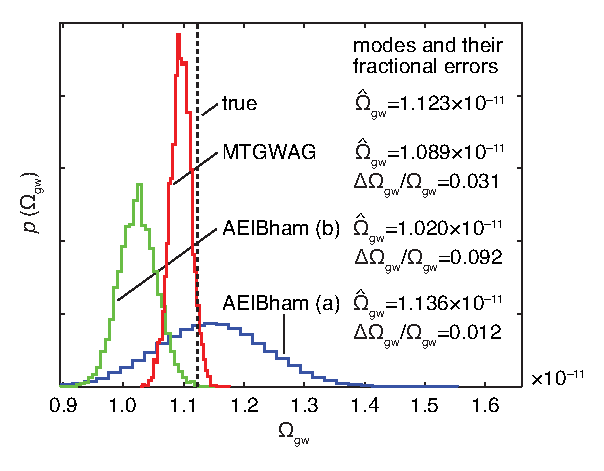
\includegraphics[width=0.5\textwidth]{stochastic_pdfs.eps}
\caption{The recovered posterior PDFs on $\Omega_{\mathrm{gw}}$ for the three analyses.
\label{fig:stochastic_pdf}}
\end{figure}


All three analyses recovered the injected value to within $10\%$.
The major difference between the analyses is the treatment of the instrumental
noise. 
The AEIBham analyses 
used analytical expressions to characterise the shape of the noise power spectra
in the $A$ and $E$ channels, such that the noise model had two unknown parameters;
the overall amplitudes of the noise PSDs.
For this it was assumed that the secondary noises were symmetrical,
which was not true of these data. It was also assumed that the GW spectrum was
flat throughout the whole band, which was not in fact the case at higher frequencies. This
may explain why the AEIBham (b) result was further from the injected
value that either the AEIBham (a) result (where the GW spectrum was indeed
a true power law throughout the whole band) or the MTGWAG result (where the 
response function had been recalibrated using the training data to take 
this into account).

The MTGWAG analyses used all three channels, and fully characterised the noise
in terms of the twelve secondary noise amplitudes (again assuming that the 
spectral shapes were fixed). It also compensated for the fact that the
GW spectrum was not a power law at high frequency by using a response function
calibrated using the training data. The recovered secondary noise amplitudes are compared to the injected
values in Table \ref{tab:MTGWAG_noise_est}. Although the individual parameters
were not well constrained, certain combinations were, and the amplitude of
the GW spectrum was recovered to within a few percent of the injected value.

\begin{table}
\begin{center}
\begin{tabular}{l@{+}l|lll}
\hline
\multicolumn{2}{l|}{Combination} & Estimated value & Injected value & Relative error \\
\hline
pm1 & pm2s & $6.503 \times 10^{-48}$ & $4.697 \times 10^{-48}$ & $0.385$ \\ 
pm1s & pm3 & $3.240 \times 10^{-48}$ & $5.375 \times 10^{-48}$ & $0.397$ \\ 
pm2 & pm3s & $6.912 \times 10^{-48}$ & $5.775 \times 10^{-48}$ & $0.197$ \\ 
pd1 & pd2s & $3.733 \times 10^{-37}$ & $3.752 \times 10^{-37}$ & $5.030 \times 10^{-3}$ \\ 
pd1s & pd3 & $3.568 \times 10^{-37}$ & $3.547 \times 10^{-37}$ & $6.082 \times 10^{-3}$ \\ 
pd2 & pd3s & $3.805 \times 10^{-37}$ & $3.804 \times 10^{-37}$ & $3.552 \times 10^{-4}$ \\ 
\hline
\end{tabular}
\end{center}
\caption{Combinations of amplitudes of secondary noises 
recovered by the MTGWAG analysis.
\label{tab:MTGWAG_noise_est}
}
\end{table} 


\section{Moving Forward: Prospects for Challenge 4 {\it Michele}}

\section{Conclusion}

\ack

\ilya{Needs updating}

SB, EKP, and JTW acknowledge support from the German Aerospace Center (DLR) and the Max-Planck Society.
MB: from NASA Grant NNG04GD52G and the NASA Center for GW Astronomy at the University of Texas, Brownsville (NAG5-13396). 
NC: NASA Grants NNG05GI69G and NNX07AJ61G.
MV: the LISA Mission Science Office and by JPL's HRDF.
DB and SF: NSF grant PHY-0601459 and the LIGO Lab.
JG: St Catharine's College, Cambridge.
IM: the Brinson Foundation, NASA grant NNG04GK98G and NSF grant PHY-0601459.
RP: the Max-Planck Society.
LW: the Alexander von Humboldt Foundation's Sofja Kovalevskaja Programme, funded by the German Federal Ministry of Education and Research.
JTW: NSF grant NSF grant PHY-0855494.
JC's, CC's and MV's work was carried out at the Jet Propulsion Laboratory, California Institute of Technology, under contract with the National Aeronautics and Space Administration.

\section*{References}

\begin{thebibliography}{99}

\bibitem{MLDC3}
%Stanislav Babak, John~G. Baker, Matthew~J. Benacquista, Neil~J. Cornish, Jeff
%  Crowder, Shane~L. Larson, Eric Plagnol, Edward~K. Porter, Michele Vallisneri,
%  Alberto Vecchio, Keith Arnaud, Leor Barack, Arkadiusz Blaut, Curt Cutler,
%  Stephen Fairhurst, Jonathan Gair, Xuefei Gong, Ian Harry, Deepak Khurana,
%  Andrzej Krolak, Ilya Mandel, Reinhard Prix, B.~S. Sathyaprakash, Pavlin
%  Savov, Yu~Shang, Miquel Trias, John Veitch, Yan Wang, Linqing Wen, and
%  John~T. Whelan.
S. Babak \& al.~2008 \textit{Class. Quant. Grav.} \textbf{25}, 184026.
%\newblock The mock lisa data challenges: from challenge 1b to challenge 3.
%\newblock {\em gr-qc/arXiv}, 0806.2110, (2008).

\bibitem{MLDC2Res}
%S.~Babak, J.~G. Baker, M.~J. Benacquista, N.~J. Cornish, J.~Crowder, C.~Cutler,
%  S.~L. Larson, T.~B. Littenberg, E.~K. Porter, M.~Vallisneri, A.~Vecchio,
%  G.~Auger, L.~Barack, A.~Blaut, E.~Bloomer, D.~A. Brown, N.~Christensen,
%  J.~Clark, S.~Fairhurst, J.~R. Gair, H.~Halloin, M.~Hendry, A.~Jimenez,
%  A.~Krolak, I.~Mandel, C.~Messenger, R.~Meyer, S.~Mohanty, R.~Nayak,
%  A.~Petiteau, M.~Pitkin, E.~Plagnol, R.~Prix, E.~L. Robinson, C.~Roever,
%  P.~Savov, A.~Stroeer, J.~Toher, J.~Veitch, J.-Y. Vinet, L.~Wen, J.~T. Whelan,
%  and G.~Woa.
S. Babak \& al.~2008 \textit{Class. Quant. Grav.} \textbf{25}, 114037.
%\newblock Report on the second mock lisa data challenge.
%\newblock In {\em Proceedings of the 7th Amaldi Conference on Gravitational Waves}, page~8, Sydney, Australia, July 2007.
%\newblock {\em arXiv:0711.2667}, (2007).

\bibitem{BabakGairPorter} Babak S, Gair J R, Porter E 2009 \textit{Class. Quant. Grav.} \textbf{26} 135004.

\bibitem{barackcutler} Barack L and Cutler C 2004 \textit{Phys. Rev.} D \textbf{69} 082005

\bibitem{mldcgwdaw2} Arnaud K A et al. (the MLDC Task Force) 2007 \textit{Class. Quant. Grav.} \textbf{24} S551

\bibitem{GAspinbbhFullPaper}
A. Petiteau, Y. Shang, S. Babak and  F. Feroz
\newblock {\em in preparation } (2009)

\bibitem{MultiNest2}
M.~Bridges F.~Feroz, M. P.~Hobson.
%\newblock Multinest: an efficient and robust bayesian inference tool for cosmology and particle physics.
\newblock {\em MNRAS}, 398:1601, (2009).


\bibitem{SMBHCornishPorter}
N.~J. Cornish and E.~K. Porter.
%\newblock The search for massive black hole binaries with lisa.
\newblock {\em Class. Quant. Grav.}, 24:5729, (2006).

\bibitem{JPLCaltech}
D. A. Brown, J. Crowder, C. Cutler, I. Mandel, M. Vallisneri
\newblock {\em  Class. Quant. Grav.}, 24:{S595}, (2007)  

\bibitem{Xspec}
K. A. Arnaud \& al.
\newblock {\em  Web}, http://heasarc.gsfc.nasa.gov/docs/xanadu/xspec/ 

\bibitem{GairMandelWen}
Gair J R, Mandel I, Wen L 2008 {\em Class. Quant. Grav.} \textbf{25} 184031.

\bibitem{SpinBBHLangHugues}
R.~N. Lang and S.~A. Hugues.
%\newblock Measuring coalescing massive binary black holes with gravitational waves : The impact of spin-induced precession.
\newblock {\em Phys. Rev. D}, 74:122001, (2006).

\bibitem{CATS}
Mandel I and Gair J R 2009 In preparation

\bibitem{keycornish} Shapiro Key~J \& Cornish~N~J, Phys. Rev. D {\bf 79} 043014 (2009).

\end{thebibliography}

\end{document}




\section{Data sets 2.1 and 2.2: The Galaxy}

Five groups submitted Galactic-binary catalogs for data sets 2.1 and 2.2:
%
\begin{description}
\item[GLIG] This collaboration of research groups at institutions in the UK, USA and New Zealand developed a Reversible-Jump Markov Chain Monte Carlo (RJ MCMC) code that can sample models with different numbers of sources; for lack of time, however, they only submitted parameter sets for the verification binaries.
\item[IMPAN] Kr\'olak and B\l aut developed an $\mathcal{F}$-statistic, template-bank--based matched-filtering search \cite{JKS98,KTV04}, and submitted parameters for 404 sources for data set 2.1.
\item[MTJPL] The Montana State--JPL collaboration used a Metropolis--Hastings Monte Carlo (MHMC) code that ran separately for overlapping frequency bands and for different hypothesized numbers of sources; model comparison was then used to determine the most probable number of sources in each band. MTJPL submitted parameter sets for 19,324 sources for data set 2.1, and 18,461 sources for 2.2.
\item[PrixWhelanAEI] Prix and Whelan developed an $\mathcal{F}$-statistic,
template-bank--based matched-filtering search using a hierarchical
scheme that enforced trigger coincidence between TDI observables,
followed by a coherent follow-up using noise-orthogonal TDI
combinations \cite{prixwhelan}. They submitted parameter sets for 1777 sources for data set 2.1, and 1737 sources for 2.2.
\item[UTB] Nayak, Jimenez and Mohanty used a tomographic reconstruction technique and submitted parameters for 3862 sources in data set 2.1.
\end{description}
%
Evaluating the performance of these searches brings up several problems of principle: while we know that many of the $\sim 30$ million Galactic sources that were injected into the data sets cannot be recovered because they are (relatively) too weak, we do not have a precise estimate of how many sources should be recoverable. Thus, the notion of false dismissal is not well defined. To make matters worse, the notion of false positive is also ill defined, because a single recovered source can provide a good fit to the blended signal from several injected sources, which may well be the ``right'' answer with the knowledge we have, since it is the best fit to the data with the smallest numbers of parameters.

The task force devoted considerable time to the analysis of Galactic-binary searches, and we do not have space here to describe all the treatments that we applied to the data. Instead we will limit our report to techniques that pair up individual recovered sources with individual sources from the challenge key, with the understanding that this will overestimate the number of false positives, and say nothing about false dismissals.
%
%\begin{figure}
%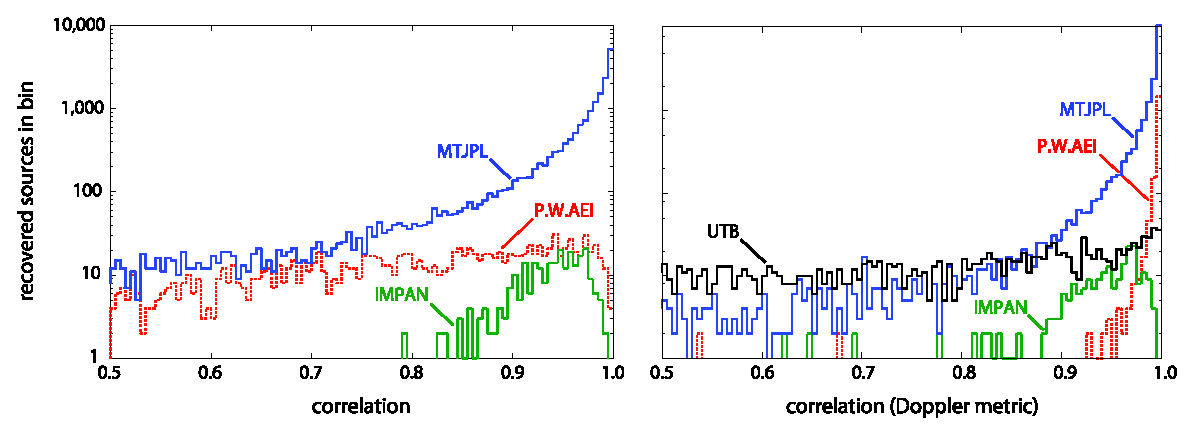
\includegraphics[width=\textwidth]{Correlations-2}
%\vspace{-18pt}
%\caption{Signal-correlation analysis of Challenge-2.1 Galactic-binary catalogs (histogram, with bin fractions on logarithmic scale).  Left panel: reported and injected sources associated by correlation; right: associated by Doppler metric.\label{fig:correlation}}
%\vspace{-6pt}
%\end{figure}

One way to proceed is to associate the reported and injected sources that have the strongest signal correlation (in terms of the noise-weighted inner product between the injected and recovered sources), limiting the search to the bright injected sources (with optimal $\mathrm{SNR} > 2$) that could in principle have been found: in the left panel of figure \ref{fig:correlation} we show the distribution of correlations generated with this procedure for data set 2.1.
Detections with the highest correlations can be considered reliable, while those with the lowest correlations probably represent spurious associations.

Another procedure is to associate the reported and injected sources that minimize the \emph{Doppler distance} that spans the frequency--sky-location subspace of the full parameter space, and automatically maximizes correlation over the \emph{extrinsic parameters} (amplitude, polarization, inclination, initial phase): the right panel of figure \ref{fig:correlation} shows the resulting distribution of correlations. The UTB entry, which includes frequency and sky position but not the extrinsic parameters, can only be plotted this way. Generally, this is a softer criterion, and all searches yield better correlations by this measure (especially the PrixWhelanAEI entry,
whose long-wavelength approximation for the LISA response is prone to extrinsic-parameter errors).
%
\begin{figure}
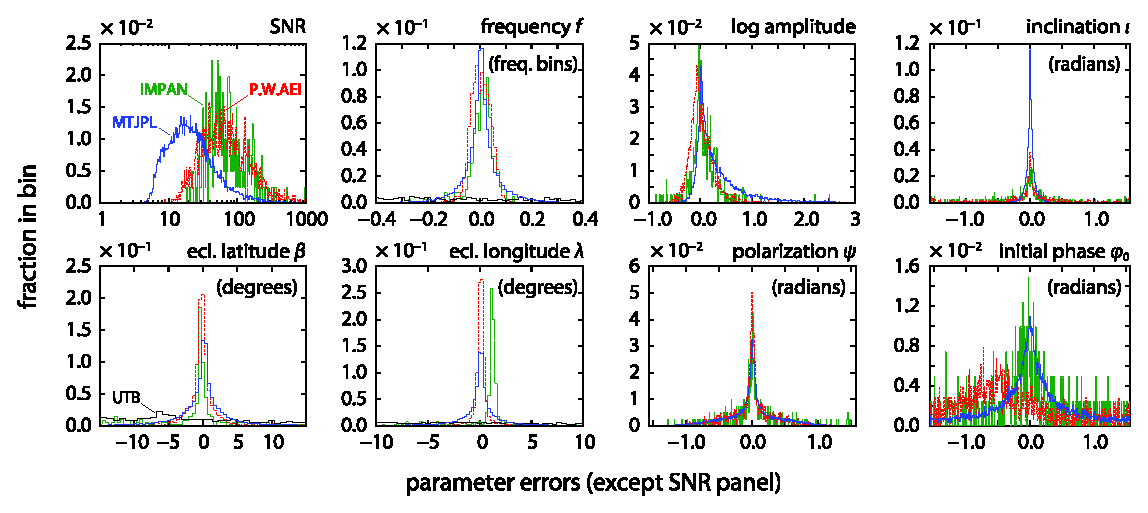
\includegraphics[width=\textwidth]{Errors-b-2}
\vspace{-18pt}
\caption{Recovered SNRs and intrinsic and extrinsic parameter errors for Challenge-2.1 Galactic-binary catalogs (histogram). True sources and templates are associated by correlation, except for the UTB catalog, for which they are associated by Doppler metric. See \cite{mldcgwdaw2} for details on the assumed Galactic-binary waveforms.\label{fig:paramerrors}}
\vspace{-6pt}
\end{figure}

Figure \ref{fig:paramerrors} shows the SNRs of the recovered sources and the errors for the intrinsic and extrinsic parameters, computed after associating sources by correlation (and by Doppler metric only for the UTB entry), again for data set 2.1. The errors in frequency are in most cases within a small fraction of a Fourier bin, and the errors in sky position are within a few degrees; by contrast, the errors in the amplitude and in the (extrinsic) orientation angles are larger. The $\phi_0$ graph for the PrixWhelanAEI suggests a systematic error in the definition of initial phase.

Altogether, these challenges demonstrated a solid capability in analyzing signals from the Galaxy and resolving a large number of binaries. As we mentioned, deciding how well they were recovered is not an easy question to answer, because of the difficulty of defining (at least operationally) a notion of \emph{identity} for recovered sources. These problems deserve careful attention in the future.

\section{Data set 2.2: MBH binaries (over the Galaxy)}

Four groups reported parameter sets for the MBH binaries in data set 2.2:
\begin{description} 
\item[AEIse] Babak and Porter used an $\mathcal{F}$-statistic, template-bank--based matched-filtering search, followed by an MCMC stage.
\item[MTAEI] Cornish and Porter used an MHMC matched-filtering search with a \emph{frequency-annealed} scheme where shorter, lower-frequency templates are used in the initial phases of the search and then progressively extended \cite{cornishporter}.
\item[JPLCT] The JPL--CIT collaboration used a three-stage pipeline consisting of a track search in the time--frequency (TF) plane, followed by template-bank--based matched filtering, and by an MCMC refinement \cite{brown}.
\item[LisaFrance] The French collaboration used a TF track search alone, and therefore reported only mass and time-of-coalescence parameters.
\end{description}
All the four MBH binaries in the data set (MBH-1, 2, 4 and 5, with total optimal SNRs $\sim$ 2583, 25, 174 and 117) were positively detected by AEIse, MTAEI, and JPLCT; the TF method used by LisaFrance identified MBH-1 and 4, but not MBH-2, and could report only a time of coalescence for MBH-5.
%
\begin{table}
\caption{\label{tab:mbh1}%
Recovered SNRs and parameter errors for MBH-1. Here $M_c \equiv (m_1 m_2)^{3/5} / (m_1 + m_2)^{1/5}$ and $\mu = m_1 m_2 / (m_1 + m_2)$ are the chirp and reduced masses; $t_c$ and $\phi_c$ are the time and GW phase at coalescence; $\beta$ and $\lambda$ are the ecliptic latitude and longitude; $D$ is the luminosity distance; $\iota$ and $\psi$ are the inclination and polarization angles (see \cite{mldcgwdaw2} for details). All errors on angles are given in radians; the true (optimal) SNR is \textbf{2583.42}.}
\small%
\begin{tabular}{@{}l|r@{\;}r@{\;}r@{\;}r@{\;}r@{\;}r@{\;}r@{\;}r@{\;}r@{\;}r}
\br
           & SNR & $\Delta M_c/M_c$ & $\Delta \mu/\mu$ & $\Delta t_c/t_c$ & $\Delta \beta$ & $\Delta \lambda$ & $\Delta D / D$ & $\Delta \iota$ & $\Delta \psi$ & $\Delta \phi_c$ \\
           &     & $\times 10^{-5}$ & $\times 10^{-5}$ & $\times 10^{-6}$ & $\times 10^{-1}$ & $\times 10^{-2}$ & $\times 10^{-2}$ & $\times 10^{-2}$ & $\times 10^{-1}$ & $\times 10^{-1}$ \\
\mr
AEIse      & 2247.60 &  147.0 & 3386.2 & 19.0 & $-5.07$ & $-82.1$ & 77.8 & $-6.86$ &  13.8 & $-6.82$ \\
MTAEI      & 2583.34 &    7.9 &    9.1 &  3.6 & 1.65 &  $-1.2$ &  3.5 &  4.94 &   1.2 & $-7.70$ \\
JPLCT      & 2582.42 &   27.5 &   28.7 & 16.0 & 4.81 &  12.2 & 12.3 & $-3.19$ & $-12.1$ &  7.45 \\
lisaFrance & \multicolumn{1}{c}{--} & 2944.6 &   72.7 & 67.8 & \multicolumn{1}{c}{--}    &  \multicolumn{1}{c}{--}   & \multicolumn{1}{c}{--}   & \multicolumn{1}{c}{--}    & \multicolumn{1}{c}{--}    &  \multicolumn{1}{c}{--}   \\
\br
\end{tabular}
% note: I'm inverting the \theta errors because we quote \beta
\end{table}
%
\begin{table}
\vspace{-9pt}
\caption{Recovered SNRs and parameter errors for MBH-4, given as in table \ref{tab:mbh1}. The true (optimal) SNR is \textbf{174.12}.\label{tab:mbh4}}
\small%
\begin{tabular}{@{}l|r@{\;}r@{\;}r@{\;}r@{\;}r@{\;}r@{\;}r@{\;}r@{\;}r@{\;}r}
\br
           & SNR & $\Delta M_c/M_c$ & $\Delta \mu/\mu$ & $\Delta t_c/t_c$ & $\Delta \beta$ & $\Delta \lambda$ & $\Delta D / D$ & $\Delta \iota$ & $\Delta \psi$ & $\Delta \phi_c$ \\
           &     & $\times 10^{-6}$ & $\times 10^{-4}$ & $\times 10^{-6}$ & $\times 10^{-2}$ & $\times 10^{-2}$ & $\times 10^{-3}$ & $\times 10^{-3}$ & $\times 10^{-3}$ & $\times 10^{-1}$ \\
\mr
AEIse       & 81.38     &   1396.3  &  149.9 &   3.4 & $-12.5$ & $ 104.7$ &  574.0 &  $  3.5$ &   $-185.4$ & $  8.1$ \\
MTAEI       & 174.13    &    148.8  &   21.3 &   2.1 & $2.4$ & $   2.1$ &   15.1 &  $  2.8$ &   $  -7.5$ & $  1.7$ \\
            & 174.11    &     17.1  &   20.5 &  33.3 & $-42.4$ & $-310.6$ &   16.7 &  $-13.7$ &   $-146.3$ & $ -6.3$ \\
JPLCT       & 174.11    &      4.2  &    9.5 &   2.1 & $7.8$ & $   9.6$ &    1.2 &  $  1.3$ &   $ -21.3$ & $ -5.4$ \\
            & 174.12    &    124.7  &    9.0 &  35.4 & $-47.3$ & $-302.9$ &    6.3 &  $-12.4$ &   $1436.4$ & $-12.4$ \\
lisaFrance  & \multicolumn{1}{c}{--}        &  34394.1  & 1804.1 & 280.8 &  \multicolumn{1}{c}{--}    &  \multicolumn{1}{c}{--}      &  \multicolumn{1}{c}{--}    &    \multicolumn{1}{c}{--}   &   \multicolumn{1}{c}{--}       & \multicolumn{1}{c}{--}      \\
\br
\end{tabular}
\vspace{-6pt}
\end{table}

Tables \ref{tab:mbh1} and \ref{tab:mbh4} show fractional parameter errors for MBH-1 and 4, together with the SNR recovered by the best-fit candidates, computed as 
%
\begin{equation}
\mathrm{SNR}_\mathrm{best}  = \frac{(A_\mathrm{true}|A_\mathrm{best}) + (E_\mathrm{true}|E_\mathrm{best})}
{\sqrt{(A_\mathrm{best}|A_\mathrm{best}) + (E_\mathrm{best}|E_\mathrm{best})}},
\end{equation}
%
with $(\cdot|\cdot)$ the usual noise-weighted inner product, and $A = (2X - Y - Z)/3$ and $E = (Z-Y)/\sqrt{3}$ two noise-orthogonal TDI observables (see, e.g., \cite{VCT}). Table \ref{tab:mbh1} shows that the JPLCT search for MBH-1 locked onto a secondary probability maximum with $\mathrm{SNR}_\mathrm{best}$ only slightly lower than the optimal value, but with sky positions off by several degrees, which led also to errors in the other parameters. The JPLCT authors conjecture that this was caused by first subtracting a rough MBH-1 model from the data, then subtracting the resolvable Galactic binaries, and finally refining the MBH search.

MBH-4 (table \ref{tab:mbh1}) is an interesting example of a ``true'' bimodal probability distribution for the source parameters. MTAEI and JPLCT each submitted two candidates, placed at rather different sky locations, quoting relative probability ratios of 1:1 and 1.18:1. In this case, it was probably the sky position and orientation of this source that conspired to degrade LISA's positional sensitivity, since they resulted in a very weak signal in one of the noise-orthogonal observables.

Altogether, this challenge demonstrated a solid capability in the detection and parameter estimation of nonspinning-MBH inspirals with moderate optimal SNRs, even in the presence of a strong Galactic background, at least if the inspirals can be considered close to our idealized model: circular and adiabatic with negligible spin effects. These restrictions are being relaxed for the upcoming Challenge 3.

\section{Data sets 1.3.X: EMRIs}

Three groups reported parameter sets for the EMRIs in data sets 1.3.1--1.3.4 (but none for 1.3.5). No group tackled the problem of detecting these systems in data set 2.2 (on top of the Galactic background).
%
\begin{description}
\item[BBGP] Babak and colleagues used an MCMC matched-filtering search that modeled the signal with a sequence of progressively longer templates (a \emph{time-annealed} scheme).
%
\item[EtfAG] Gair, Mandel and Wen used a TF track search that (for now) targeted only the intrinsic parameters and sky position \cite{gair}.
%
\item[MT] Cornish used an MHMC matched-filtering search, running it in parallel on individual month-long segments that were subsequently strung together.
\end{description}
%
Table \ref{tab:emri} shows typical recovered SNRs and errors. A comparison of the optimal and recoved SNRs indicates that the matched-filtering searches locked on several secondary probability maxima with similar probabilities. Still, the recovered SNRs correspond to solid detections with exceedingly low false-alarm probabilities. The errors are quoted as fractions of the allowed parameter ranges, and they are quite large. Intriguingly, the TF search was the most accurate in determining the sky position.

Altogether, these challenges demonstrated a positive capability of detecting EMRIs, at least if their signals are similar in complexity to the \emph{kludge} waveforms used in this challenge \cite{mldcgwdaw2}; however, the prospects for accurate parameter estimation are still uncertain, and a good focus for further challenges.
%
\begin{table}
\caption{Recovered SNRs and parameter errors for the EMRI signal in data set 1.3.1. Here $\beta$ and $\lambda$ are the ecliptic latitude and longitude; $\theta_K$, $\phi_K$, and $a$ set the orientation and magnitude of the central-BH spin; $\mu$ and $M$ are the compact-object and central-BH masses; $\nu_0$ is the initial radial orbital frequency; $e_0$ is the initial eccentricity; and $D$ is the luminosity distance.
All errors are given as \emph{fractions of the allowed prior range} for the corresponding parameters (0.15 for $e_0$), except for $\nu_0$ and $D$. Not all parameters are shown. See \cite{mldcgwdaw2} for details on the assumed EMRI waveforms. The true (optimal) SNR is \textbf{130.98}.\label{tab:emri}}
\small%
\lineup
\begin{tabular}{@{}l@{\;}|@{\;}l@{\;}@{\;}l@{\;}l@{\;}l@{\;}l@{\;}l@{\;}l@{\;}l@{\;}l@{\;}l@{\;}l@{\;}l@{}}
\br
& SNR & \multicolumn{1}{c}{$\delta \beta$} & \multicolumn{1}{c}{$\delta \lambda$} & \multicolumn{1}{c}{$\delta \theta_K$} & \multicolumn{1}{c}{$\delta \phi_K$} & \multicolumn{1}{c}{$\delta a$} & \multicolumn{1}{c}{$\delta \mu$} & \multicolumn{1}{c}{$\delta M$} & \multicolumn{1}{c}{$\frac{\Delta \nu_0}{\nu_0}$} & \multicolumn{1}{c}{$\delta e_0$} & \multicolumn{1}{c}{$\frac{\Delta D}{D}$} \\
\mr
BBGP    & 74.86  & $-0.33 $   & $-0.0095$   & $-0.13 $ & $-0.076$ & $\m 0.28 $ & $-0.15$   & $-0.51$   & $\m 0.017  $ & $\m 0.21 $ &  $-1.21$ \\
        & 72.96  & $-0.32 $   & $\m 0.011 $ & $-0.15 $ & $-0.078$ & $\m 0.27 $ & $-0.15$   & $-0.51$   & $\m 0.017  $ & $\m 0.21 $ &  $-1.22$ \\
        & 72.52  & $-0.28 $   & $\m 0.025 $ & $-0.063$ & $-0.036$ & $\m 0.41 $ & $-0.17$   & $-0.35$   & $-0.009  $   & $\m 0.29 $ &  $-2.15$ \\
        & 72.49  & $-0.28 $   & $\m 0.025 $ & $-0.063$ & $-0.034$ & $\m 0.41 $ & $-0.17$   & $-0.36$   & $-0.009  $   & $\m 0.29 $ &  $-2.17$ \\
        & 70.59  & $-0.31 $   & $-0.020 $   & $-0.36 $ & $-0.21 $ & $\m 0.44 $ & $-0.12$   & $-0.12$   & $-0.03   $   & $\m 0.28 $ &  $-0.91$ \\
EtfAG   & \multicolumn{1}{c}{--}  & $\m 0.016$ & $\m 0.0012$ & \multicolumn{1}{c}{--}    & \multicolumn{1}{c}{--}        & $-0.082$   & $\m 0.10 $ & $-0.17$   & $\m 0.0026 $ &  $\m 0.098$ &   \multicolumn{1}{c}{--}   \\
MT      & 74.85 & $\m 0.15 $ & $\m 0.47  $ & $-0.069$ & $-0.15 $ & $-0.026$   & $\m 0.073$ & $\m 0.18$ & $\m 0.00025$  & $-0.11 $   &  $-0.71$ \\
        & 76.52  & $\m 0.084$ & $-0.49  $   & $-0.33 $ & $-0.10 $ & $-0.022$   & $\m 0.046$ & $\m 0.16$ & $\m 0.00026$ & $-0.10 $   &  $-0.70$ \\
\br
\end{tabular}
\vspace{-6pt}
\end{table}

\section{Conclusion}

We are very excited about the outcome of the first two MLDCs, which have given a convincing demonstration that a significant portion of the LISA science objectives could already be achieved with techniques that are currently in hand. Most of the research groups that participated in Challenge 1 have successfully made the transition to the greater complexity of Challenge 2. Challenge 3 (with data sets released in Jan 2008 and results due in Dec 2008) will continue to move in the direction of more realistic signals, featuring chirping Galactic binaries and precessing binaries of spinning MBHs. It will also include two new classes of signals: an isotropic primordial GW background and bursts from the cusps of cosmic strings. In addition, Challenge 1B took place between July and Dec 2007. This was a repeat of Challenge 1, conceived to provide a softer entry point for research groups new to the MLDCs. Ten collaborations (including five new institutions) participated, demonstrating increasing sophistication and proficiency in a range of LISA data-analysis techniques.

Furthermore, the MLDC conventions, file formats, and software tools (see \url{lisatools.googlecode.com}) have matured to the point where interested parties can use them to generate a variety of data sets. This enables a wealth of interesting side investigations, such as the studies of the LISA science reach that are now being undertaken by the LISA Science Team. To obtain more information and to participate in the MLDCs, see the official MLDC website (\url{astrogravs.nasa.gov/docs/mldc}) and the task force wiki (\url{www.tapir.caltech.edu/listwg1b}).

\section*{References}

\begin{thebibliography}{99}
%
\bibitem{lisa} Bender P, Danzmann P and the LISA Study Team 1998 ``Laser Interferometer Space Antenna for the Detection of Gravitational Waves, Pre-Phase A Report'' \textbf{MPQ 233} (Garching: Max-Planck-Instit\"ut f\"ur Quantenoptik) 
%
\bibitem{mldclisasymp} Arnaud K A et al. (the MLDC Task Force) 2006 \textit{Laser Interferometer Space Antenna: 6th International LISA Symp. (Greenbelt, MD, 19--23 Jun 2006)} ed Merkowitz S M and Livas J C (Melville, NY: AIP) p 619; \textit{ibid.} p 625
%
\bibitem{mldcgwdaw1} Arnaud K A et al. (the MLDC Task Force and Challenge 1 participants) 2007 \textit{Class. Quant. Grav.} \textbf{24} S529
%
\bibitem{barackcutler} Barack L and Cutler C 2004 \textit{Phys. Rev.} D \textbf{69} 082005
%
\bibitem{mldcgwdaw2} Arnaud K A et al. (the MLDC Task Force) 2007 \textit{Class. Quant. Grav.} \textbf{24} S551
%
\bibitem{JKS98}
P.\ Jaranowski, A.\ Kr\'olak, and B.\ F.\ Schutz, Phys.\ Rev.\ D
{\textbf 58}, 063001 (1998).
%
\bibitem{KTV04} A. Kr\'olak, M. Tinto, and M. Vallisneri, {\it Phys. Rev. D}, {\bf 70},
022003 (2004).
%
\bibitem{prixwhelan} Prix R and Whelan J T 2007 \textit{Class. Quant. Grav.} \textbf{24} S565; \textit{Poster} \url{www.ligo.caltech.edu/docs/G/G070462-00.pdf}
%
\bibitem{cornishporter} Cornish N J and Porter E K 2007 \textit{Class. Quantum Grav.} \textbf{24} 5729--5755
%
\bibitem{brown} Brown D A, Crowder J, Cutler C, Mandel I and Vallisneri M 2007 \textit{Class. Quant. Grav.} \textbf{24} S595
%
\bibitem{VCT} Vallisneri M, Crowder J and Tinto M 2007 ``Sensitivity and parameter-estimation precision for alternate LISA configurations'' \textit{Preprint} arxiv.org/0710.4369 
%
\bibitem{gair} Gair J R, Mandel I and Wen L 2007 Proc. 7th Amaldi Conf. on Gravitational Waves (Sydney, 8--14 July 2007), submitted. \textit{Preprint} arXiv:0710.5250
%
\end{thebibliography}

